\chapter{Evaluation}
The following chapter presents the results of some experiments done with the \gls{icds}.
Evaluation has been done in different areas to give a complete impression of how the \gls{icds} performs.
In the first section some general findings will be described that affect overall performance.
Afterwards the test environment and setup of the IMSI catcher is discussed.
The last two sections evaluate the \gls{icds} against a configured catcher, first to test the individual rules and second against the attacks that were listed earlier.

\section{Performance Evaluation}
In order to evaluate general performance it has to be considered that the \gls{icds} can be deployed in different environments.
To reflect different compositions and densities of base stations form different areas, four distinct data sets will be used for the experiments in this section.
The data sets have been taken in areas surrounding the city of Freiburg.
Table shows some of data sets' key values.

\begin{table}
\centering
\begin{tabular}{llrr}
\toprule
Name					&Description					&Number of BTS	&Scan Duration\\
\midrule
\texttt{cdb}			&CBD around the area of			&54				&6:13		\\
						&Bertholdsbrunnen				&				&			\\
\texttt{airport}		&Airport and university area	&68				&6:25		\\
						&around Georges Koehler Allee	&				&			\\
\texttt{ind\_park}		&Industrial park Haid in 		&53				&4:52		\\
						&Freiburg West,  Hausener Weg	&				&			\\
\texttt{house\_area}	&Housing area at the rim of 	&22				&3:59		\\
						&Freiburg Zähringen, Thuner Weg	&				&			\\
\bottomrule
\end{tabular}
\caption{Key values of the data sets used for performance tests.}
\label{tab:key_data}
\end{table}

Apart from nodes from the four public \gls{gsm} providers E-Plus, T-Mobile, Vodafone and O2, nodes from Deutsche Bahn also occur in these scans.
These nodes form a private network used for internal communications by Deutsche Bahn.
They are identified by their broadcast name 'DB Systel GSM-R' and their frequency which is outside the regular bands.
Since the distribution of these nodes is very sparse, only one node can be found in each scan they yield a false positive for no neighbouring nodes can be discovered.
These nodes are not relevant to subscribers because they are not able to connect to them.
Therefore they will be ignored and factored out for the remainder of this evaluation.

\subsection{Scan Duration}
\begin{figure}
\centering
\begin{tikzpicture}
\begin{axis}[
	width=\textwidth,
	height=0.3\textheight,
	xlabel=Total BTS, 
	ylabel=Scan duration in s,
	xticklabel style={/pgf/number format/1000 sep=}
	]
	\addplot [mark=*,blue] plot coordinates {
		(68, 385)
		(54, 373)
		(53, 292)
		(22, 239)
	};
\end{axis}
\end{tikzpicture}
\caption{Scan durations for the sample data sets.}
\label{fig:durations}
\end{figure}
Table \ref{tab:key_data} shows that the times for scans in the Freiburg area can differ by large amounts depending on how many base stations are scanned.
Generally said it takes longer the more dense the base station distribution is in the scanned area.
This is however not the only factor, as Figure \ref{fig:durations} visualises.
If the scan duration would only depend on the number of base station scanned, a linear growth could be expected.

There is a large increase in scan duration between the \texttt{ind\_park} and the \texttt{cbd} data sets although only one more base station was detected.
This jump can be explained considering the context of the scan.
The scans were done on a Saturday between 14:00 and 16:00.
The Freiburg CBD was crowded at the time of the scan as was the university campus due to an event held there.
Contrary to that the industrial park area was very calm, as was the housing area.
Whenever the \gls{icds} discovers a \gls{bts} it needs to wait until all system information messages are gathered before it can continue scanning for further base stations.
In a crowded area reception is far worse due to radio inference therefore it takes longer to accumulate the information needed resulting in increased scanning times.

A crowded area with high density of \glspl{bts} could be seen as a worst case for scan duration.
Re-evaluation of a base station based on its own parameters thus occurs only every 7 minutes in this worst case.
This is an inherent problem to the approach of scanning and updating all base stations and not only monitoring a subset from a single provider.
If an IMSI catcher replaces a base station directly after it was scanned, it could take up to 7 minutes until it is discovered.
To lessen this threat, if the \gls{icds} is used in user mode, the base station with the strongest reception is scanned again, to eliminate the possibility of having been taken over and not being detected.

\subsection{Cell ID Databases}
The usefulness of the Cell ID Rule is subject to the completeness of the database that is used.
That is even more so since a database with a low coverage will yield false positives, \eg legitimate base stations will be evaluated as being IMSI catchers because they are not found in the database.

The coverage for the OpenCellID database and the Google Mobile Maps service evaluated against the data sets can be seen in Table \ref{tab:coverage}.
\begin{table}
\centering
\begin{tabular}{lrrcrrcrrcrr}
\toprule
& \multicolumn{2}{c}{\texttt{cdb}} &\phantom{a}& \multicolumn{2}{c}{\texttt{airport}} &\phantom{a} & \multicolumn{2}{c}{\texttt{ind\_park}}&\phantom{a} & \multicolumn{2}{c}{\texttt{house\_area}}\\
\cmidrule{2-3} \cmidrule{5-6} \cmidrule{8-9} \cmidrule{11-12}
&Cov.&Time&	&Cov.&Time&	&Cov.&Time&	&Cov.&Time\\
\midrule
Google&		1.00&5&	&0.99&8&	&1.00&5&	&1.00&2\\
OCID&		0.57&51&	&0.58&68&	&0.58&55&	&0.41&19\\
\bottomrule
\end{tabular}
\caption{Coverage for Google Mobile Maps and OpenCellID on the data sets with the time needed in s for fetching the information.}
\label{tab:coverage}
\end{table}
Google Mobile Maps service scored a complete coverage on all the data sets while Open Cell ID could cover about half the nodes in the different sets.
The reason the Google service had only a 99\% coverage on the \texttt{airport} data set is that base station that has not been found was the one operated by the chair of communication systems, therefore it can be factored out.
The OpenCellID database is not a good source of information for this project as is shown by its coverage scores.
However it must be said that these two services are intended for localisation and thus do not have the demand to yield a complete coverage of all the base stations in the area.
Therefore it must be kept in mind when using this rule for analysis that false positives might still be brought forth.
What can be said though is that a base station that has been found may only be subject to a type of attack that replaces an existing base station and can thus be investigated more specifically.

\subsection{PCH Scans}
In order to establish a baseline on what to expect from the \gls{pch} scans different measurements have been done.
Table \ref{tab:pagings} shows scans that have been done in three different areas.
In each area the cell with the strongest reception for each provider was chosen as a representative for the respective provider.
The duration of each scan was set to 60\;s, while the values in the table have been averaged for 10\;s since this is the unit the \gls{icds} is using.

A comparison of the results suggests that the different providers also have different policies when to page.
Vodafone has about six times the paging rate O$_{2}$ has but only half the Immediate Assignments.

Another scan was also done on the IMSI catcher.
No Paging Messages or Immediate Assignments were detected although \glspl{ms} were connected to it.
That was to be expected as formerly discussed in Section \ref{sec:paging} because the IMSI catcher is not actually part of the providers network and thus cannot receive and forward paging requests.
\begin{table}
\centering
\begin{tabular}{lrrcrrcrr}
\toprule
& \multicolumn{2}{c}{\texttt{house\_area}} &\phantom{a}& \multicolumn{2}{c}{\texttt{cbd}} &\phantom{a} & \multicolumn{2}{c}{\texttt{airport}}\\
\cmidrule{2-3} \cmidrule{5-6} \cmidrule{8-9}
&Pagings&IAs&	&Pagings &IAs.&	&Pagings&IAs.\\
\midrule
T-Mobile&		89&3&	&75&3&	&109&4\\
E-Plus&		119&1&	&67&2&	&70&1\\
Vodafone&		776&6&	&720&5&	&712&6\\
O2&		117&9&	&106&16&	&94&11\\
\bottomrule
\end{tabular}
\caption{Number of Pagings and Immediate Assignments (per 10\;s) for the four German providers at different locations.}
\label{tab:pagings}
\end{table}

\section{IMSI Catcher Detection}
Before using an IMSI catcher for testing purpose or a launching an OpenBTS base station it should be ensured that licenses for the specific frequencies that are used, have been obtained.
This way it can be ensured that the operation does not interfere with regular radio communication.
Extra care should be taken when configuring the IMSI catcher to simulate a real base station to reject incoming connections when the experiments are done within a radio sealed room.
Otherwise subscribers might get caught by the catcher and might not be able to initiate calls.
How this can be done for the Open Source IMSI Catcher that is used to test the \gls{icds} is explained in the next section.

\subsection{Open Source IMSI Catcher}
The rules themselves cannot be tested without an active IMSI catcher.
For this purpose the Open Source IMSI Catcher \cite{dennis} is used.

This project builds up an IMSI catcher using only Open Source systems and freely available hardware so it can basically be used by anybody.
On the hardware side a computer running a Linux operating system is used, as well as the \gls{usrp} as the radio transmitter.
The \gls{usrp} allows the signal processing for radio transmissions to be done in software, therefore it can be used for a multitude of purposes and protocols.
Some hardware modifications have to be done to the device to empower it to send and receive data on the frequency bands used for \gls{gsm} communication.
An external clock needs to be used since \gls{gsm} operations are very time critical.
Figure \ref{fig:setup} shows the Open Source IMSI Catcher and the \gls{icds} side by side.

On the software side GNU Radio\footnote{GNU Radio Project Wiki, \url{http://gnuradio.org/redmine/projects/gnuradio/wiki} [Online; Accessed 05.2012]}, OpenBTS\footnote{OpenBTS Project Wiki, \url{http://wush.net/trac/rangepublic} [Online; Accessed 05.2012]} and Asterisk\footnote{Asterisk, \url{http://www.asterisk.org} [Online; Accessed 05.2012]} are used to achieve the functionality provided by a IMSI catcher.
\begin{figure}
\caption{Open Source IMSI Catcher (left) with USRP (black) and external clock (blue) and the ICDS (right) with the Motorola C123 connected.}
\label{fig:setup}
\end{figure}
The raw data that is received by the \gls{usrp} is sent to the GNU Radio component which works as a software side interface to the \gls{usrp}.
This data is taken by the OpenBTS software that emulates base station behaviour and has an integrated module simulating a \gls{vlr} and handing out \glspl{tmsi}.
OpenBTS implements an open source version of the \gls{gsm} stack with the goal to provide cheap access points to the \gls{gsm} network in areas with bad coverage.
The user accounts are as well as encoding of voice data and recording of calls is handled inside the Asterisk software, basically combining the \gls{trau}, \gls{hlr} and authentication centre of a real \gls{gsm} network.
Calls are routed from here on to the \gls{voip} network of the university.

Since we do not want to actually connect to the IMSI catcher, the Asterisk part and user configuration will be omitted here.
The parameters necessary to simulate a \gls{gsm} cell have to be set inside the \texttt{OpenBTS.conf}.
Figure \ref{fig:openbts_parameters} shows an annotated example for a configuration simulating a T-Mobile cell.
\begin{figure}
\hspace*{\dimexpr\fboxsep+\fboxrule}% 
\begin{minipage}{\dimexpr\textwidth-4\fboxsep-2\fboxrule} 
\begin{lstlisting}
#Do not let people connect
Control.OpenRegistration 0

#Basic cell parameters
GSM.MCC 262			GSM.ARFCN 54
GSM.MNC 01			GSM.ShortName T-Mobile
GSM.LAC 29184		
GSM.CI 61858
	
#Transmission strength ranging from 0 to 23
GSM.PowerAttenDB 20

#Neighbouring cell list, space separated
GSM.Neighbours 69 53 20

#Force location Updates, multiple of 6 minutes
GSM.T3212 1
\end{lstlisting}
\end{minipage}
\caption{Excerpt of a \texttt{OpenBTS.conf}.}
\label{fig:openbts_parameters}
\end{figure}
\texttt{Control.OpenRegistration} is explicitly set to 0 which prevents anyone from connecting to the IMSI catcher since connections are not part of the test and we do not want to interfere with other peoples' communications in the area.
More precisely this will only let users connect that have been set up in the \texttt{sip.conf} of the Asterisk server.
Only the test phone does have a valid account.

\begin{figure}
\centering
\subfigure[Connected cell information.]{}
\subfigure[Neighbouring cell measurements.]{}
\caption{Nokia 3310 NetMonitor screenshots.}
\label{fig:netmonitor}
\end{figure}

\subsubsection{Nokia 3310}
To get feedback on whether the IMSI catcher is working as intended or see if an attack succeeded a Nokia 3310 phone can be used.
Nikia has a software called NetMonitor\footnote{ofo} that can be used to measure base stations in the perimeter and gives feedback when the \gls{ms} is going to switch to a new cell.
This NetMonitor consists of several pages, of which the first shows the active cell that the phone is connected to.
On the following pages neighbouring cell measurements can be seen ordered by a score that is used by the phone to determine when and if to change the cell.
Figure \ref{fig:netmonitor} shows the home screen with information on the connected cell (a) as well as the first page of the neighbouring cell measurements (b).

\subsection{Rule Evaluation}
With the environment set up we will now evaluate the individual rules.
The IMSI catcher was launched with the four different configurations shown in Table \ref{tab:err_configs}.
\begin{table}
\centering
\begin{tabular}{lllll}
\toprule
			&Conf. 1		&Conf. 2		&Conf. 3		&Conf. 4\\
\midrule
ARFCN		&50				&2				&978			&695	\\
ShortName	&T-Mobile		&Vodafone		&E-Plus			&O2		\\
MCC			&262			&262			&262			&505	\\
MNC			&01				&02				&03				&07	\\
LAC			&21010			&793			&588			&50945	\\
Cell ID		&1				&2				&3				&4		\\
Neighbours	&-				&10,11,12		&695, 20		&1022, 1001 \\
\bottomrule
\end{tabular}
\caption{Erroneous configurations for the IMSI catcher.}
\label{tab:err_configs}
\end{table}
With each of these configurations the \gls{icds} detected the catcher for various reasons:
\begin{itemize}
	\item Config 1: For this configuration the \gls{icds} detected that \gls{arfcn} 50 is not in the range registered to the provider T-Mobile.
	Apart from that the \gls{lac} differed from the ones found in the Freiburg area and thus different from the neighbouring \glspl{lac}.
	The neighbouring cell list was also empty which is a strong indication for an IMSI catcher. 
	An interesting fact to be noted here is, when an empty neighbourhood list is given to OpenBTS it still transmits a neighbourhood list containing the element '0'.
	The Neighbourhood Structure Rule triggered nevertheless since no other T-Mobile station in the area had \gls{arfcn} 0 as a neighbour, nor was it discovered during the scan.\\
	Rules triggered: LAC/Provider Mapping, Neighbourhood Structure, ARFCN/Provider Mapping, LAC Median Deviation
	\item Config 2: The detected errors within this configuration are that none of the neighbours mentioned was in range to be detected, which is very unlikely for a normal base station.\\
	Rules triggered: Neighbourhood Structure
	\item Config 3: In this configuration one of the neighbours, namely 695 is not consistent with the set provider.
	The base stations breaks up the isolated subgraph for E-Plus and is thus detected.\\
	Rules triggered: Pure Neighbourhoods
	\item Config 4:	The chosen provider is not consistent with the country set.
	Additionally another warning is thrown since the neighbourhood list only contained nodes that were only found indirectly.\\
	Rules triggered: Country/Provider Mapping, Neighbourhood Structure (warning) 
\end{itemize}
The \emph{LAC Change} and the \emph{rx Change} rules remain to be tested.
For this purpose the procedure was as follows.
At first the \gls{icds} was turned on an scanning commenced.
Afterwards the IMSI catcher was turned on, operating on the same frequency as a base station that was previously discovered.
This was repeated several times with the IMSI catcher replacing another node each time.
Table \ref{tab:par_change} summarises the findings.
The configurations used can be found in Appendix \ref{sec:config_data}.
In all cases the \gls{icds} was able to detect the IMSI catcher after about 2 minutes.
These times can vary however depending on the timing of the catcher being turned on and the time it takes for rescanning a base stations as described in the beginning of this chapter.
\begin{table}
\centering
\begin{tabular}{lrrcrrrllr}
\toprule
			&				&\multicolumn{2}{c}{rx}		&\phantom{a}	&\multicolumn{2}{c}{LAC}	&				&	&		\\
								\cmidrule{3-4} 								\cmidrule{6-7} 
Config 		&Cell			&Old	&New				&				&Old	&New				&rx det.	&LAC det.		&Time\\
\midrule
T-Mobile	&17				&-94 dB	&-55dB				&				&138	&139				&Yes		&Yes	&42 s\\
O2			&877			&-94 dB	&-55dB				&				&138	&139				&Yes		&Yes	&42 s\\
E-Plus		&877			&-94 dB	&-55dB				&				&138	&139				&Yes		&Yes	&42 s\\
Vodafone	&877			&-94 dB	&-55dB				&				&138	&139				&Yes		&Yes	&42 s\\
\bottomrule
\end{tabular}
\caption{failzor}
\label{tab:par_change}
\end{table}

\subsection{Long Term Test}
To evaluate the \emph{Location Area Database} rule a long term test has been carried out.
This has been done to find out whether base stations in the surrounding area change on a regular basis or stay the same (including their respective configurations and reception levels).
This is essential for a Location Area Database to be usable over a longer period of time.

The database itself has been built over the course of one week in Freiburg, Thuner Weg.
During this period no parameter changes were detected and the reception of base stations only varied inside a very small interval.
After that each day for another week, two scans per day were done.
One of them while the IMSI catcher was operating, the other without the device present.
This was done to evaluate if false positives or negatives occurred using the database and all the methods mentioned above over a larger period of time.
The results on a per day basis are summarised in Table \ref{tab:longterm_test}.
\begin{table}
\centering
\begin{tabular}{lllllrr}
\toprule
Date	&Time	&Catcher	&Detected	&Detected by	&False positives	&False negatives\\
\midrule
		&		&			&			&				&					&				\\
		&		&			&			&				&					&				\\
		&		&			&			&				&					&				\\
		&		&			&			&				&					&				\\
		&		&			&			&				&					&				\\
		&		&			&			&				&					&				\\
		&		&			&			&				&					&				\\
		&		&			&			&				&					&				\\
		&		&			&			&				&					&				\\
		&		&			&			&				&					&				\\
		&		&			&			&				&					&				\\
		&		&			&			&				&					&				\\
		&		&			&			&				&					&				\\
		&		&			&			&				&					&				\\
		&		&			&			&				&					&				\\
		&		&			&			&				&					&				\\
\bottomrule
\end{tabular}
\caption{Results of the long term evaluation.}
\label{tab:longterm_test}
\end{table}

\subsection{Attack Scenarios}
Since all the configuration rules have been tested we assume from this point on that the IMSI catcher is configured correctly, meaning that  parameters like the \gls{arfcn}, \gls{lac} or provider have been set up in correct and consistent way so the respective rules will not show an alarm.
Consistent parameters for the four providers in Germany can be found in Table \ref{tab:consistent_parameters}.
\begin{table}
\centering
\begin{tabular}{lllll}
\toprule
Parameter	&T-Mobile				&Vodafone			&E-Plus			&O2\\
\midrule
ARFCN		&13-49, 81-102,			&1-12, 50-80,		&975-999,		&0, 1000-1023,\\
			&122-124, 587-611		&103-121, 725-751	&777-863		&637-723\\
LAC			&21014/21015			&793				&588/138		&50945\\
MCC			&262					&262				&262			&262\\
MNC			&01						&02					&03				&07\\
\bottomrule
\end{tabular}
\caption{Consistent parameter configurations in the Freiburg area for the four German providers.}
\label{tab:consistent_parameters}
\end{table}
Note that the Cell ID can be a arbitrary value as long as it is unique in the area of reception. 
Cell IDs measured from different base stations do not follow any particular schema.
The scenarios are built after the attacks described in Section \ref{sec:attacks}.
Local information in terms of a Local Area Database was available.

\subsubsection{IMSI Catcher as a new Cell}
The first scenario will simulate the case where the catcher opened up a new cell with a good reception and forced the \gls{ms} into normal cell selection mode by disconnecting it from the current base station via a jammer.
First the IMSI catcher was turned on, faking a legitimate T-Mobile cell with a new cell ID.
Afterwards the \gls{icds} was started and a sweep scan was performed.
As soon as the cell was scanned which occurred very early since the reception was very good (-45) it was detected that this cell was not in the Local Area Database.
After the sweep scan cell IDs from Google were also fetched.
Both the Local Area Database Rule and the Cell ID Database Rule indicated a Critical status.

As a further step to simulate the case where no local information is available, the Local Area Database and Cell ID Rules were turned off.
The \gls{icds} then yielded an Ok evaluation since the configuration of the catcher cell was consistent.
The next step was to put the \gls{icds} into User Mode with T-Mobile as its fixed provider. 
It selected the IMSI catcher cell as its target cell because of the good reception level and since it's evaluation was 'Ok' an additional PCH scan was started.
No paging messages or Immediate Assignments were caught so the end result was a 'Critical' status for the IMSI catcher cell.

\subsubsection{IMSI Catcher replacing an old Cell}
The second scenario simulated the attack where the IMSI catcher replaces a base station with a bad reception in the neighbourhood of the cell the \gls{ms} is connected to.
This way the reception drastically improves on that particular frequency suggesting to the \gls{ms} that the subscriber moved to the close perimeter of that \gls{bts} and initiating a handover.
Figure \ref{fig:takeover_attack} illustrates this particular attack.
The station with the \gls{arfcn} 42 has the lowest reception with its signal to noise ratio of -95\,dB.
In this particular scenario the \gls{ms} would first connect to the station on 23 because of its good reception.
After that the IMSI catcher is turned on also on \gls{arfcn} 42.
Due to its location it has the best reception level of all the available base station.
Since it replaced station 42 it is most likely in the neighbourhood list of 23.
When the \gls{ms} conducts a neighbouring cell measurement it will find that the catcher has the best reception and will switch to it.
Disconnection and cell re-selection of the \gls{ms} could also be achieved instantly by jamming \gls{arfcn} 23.
Since the catcher sends a different \gls{lac} the \gls{ms} will send a location update to the IMSI catcher announcing its presence.
\begin{figure}
\centering
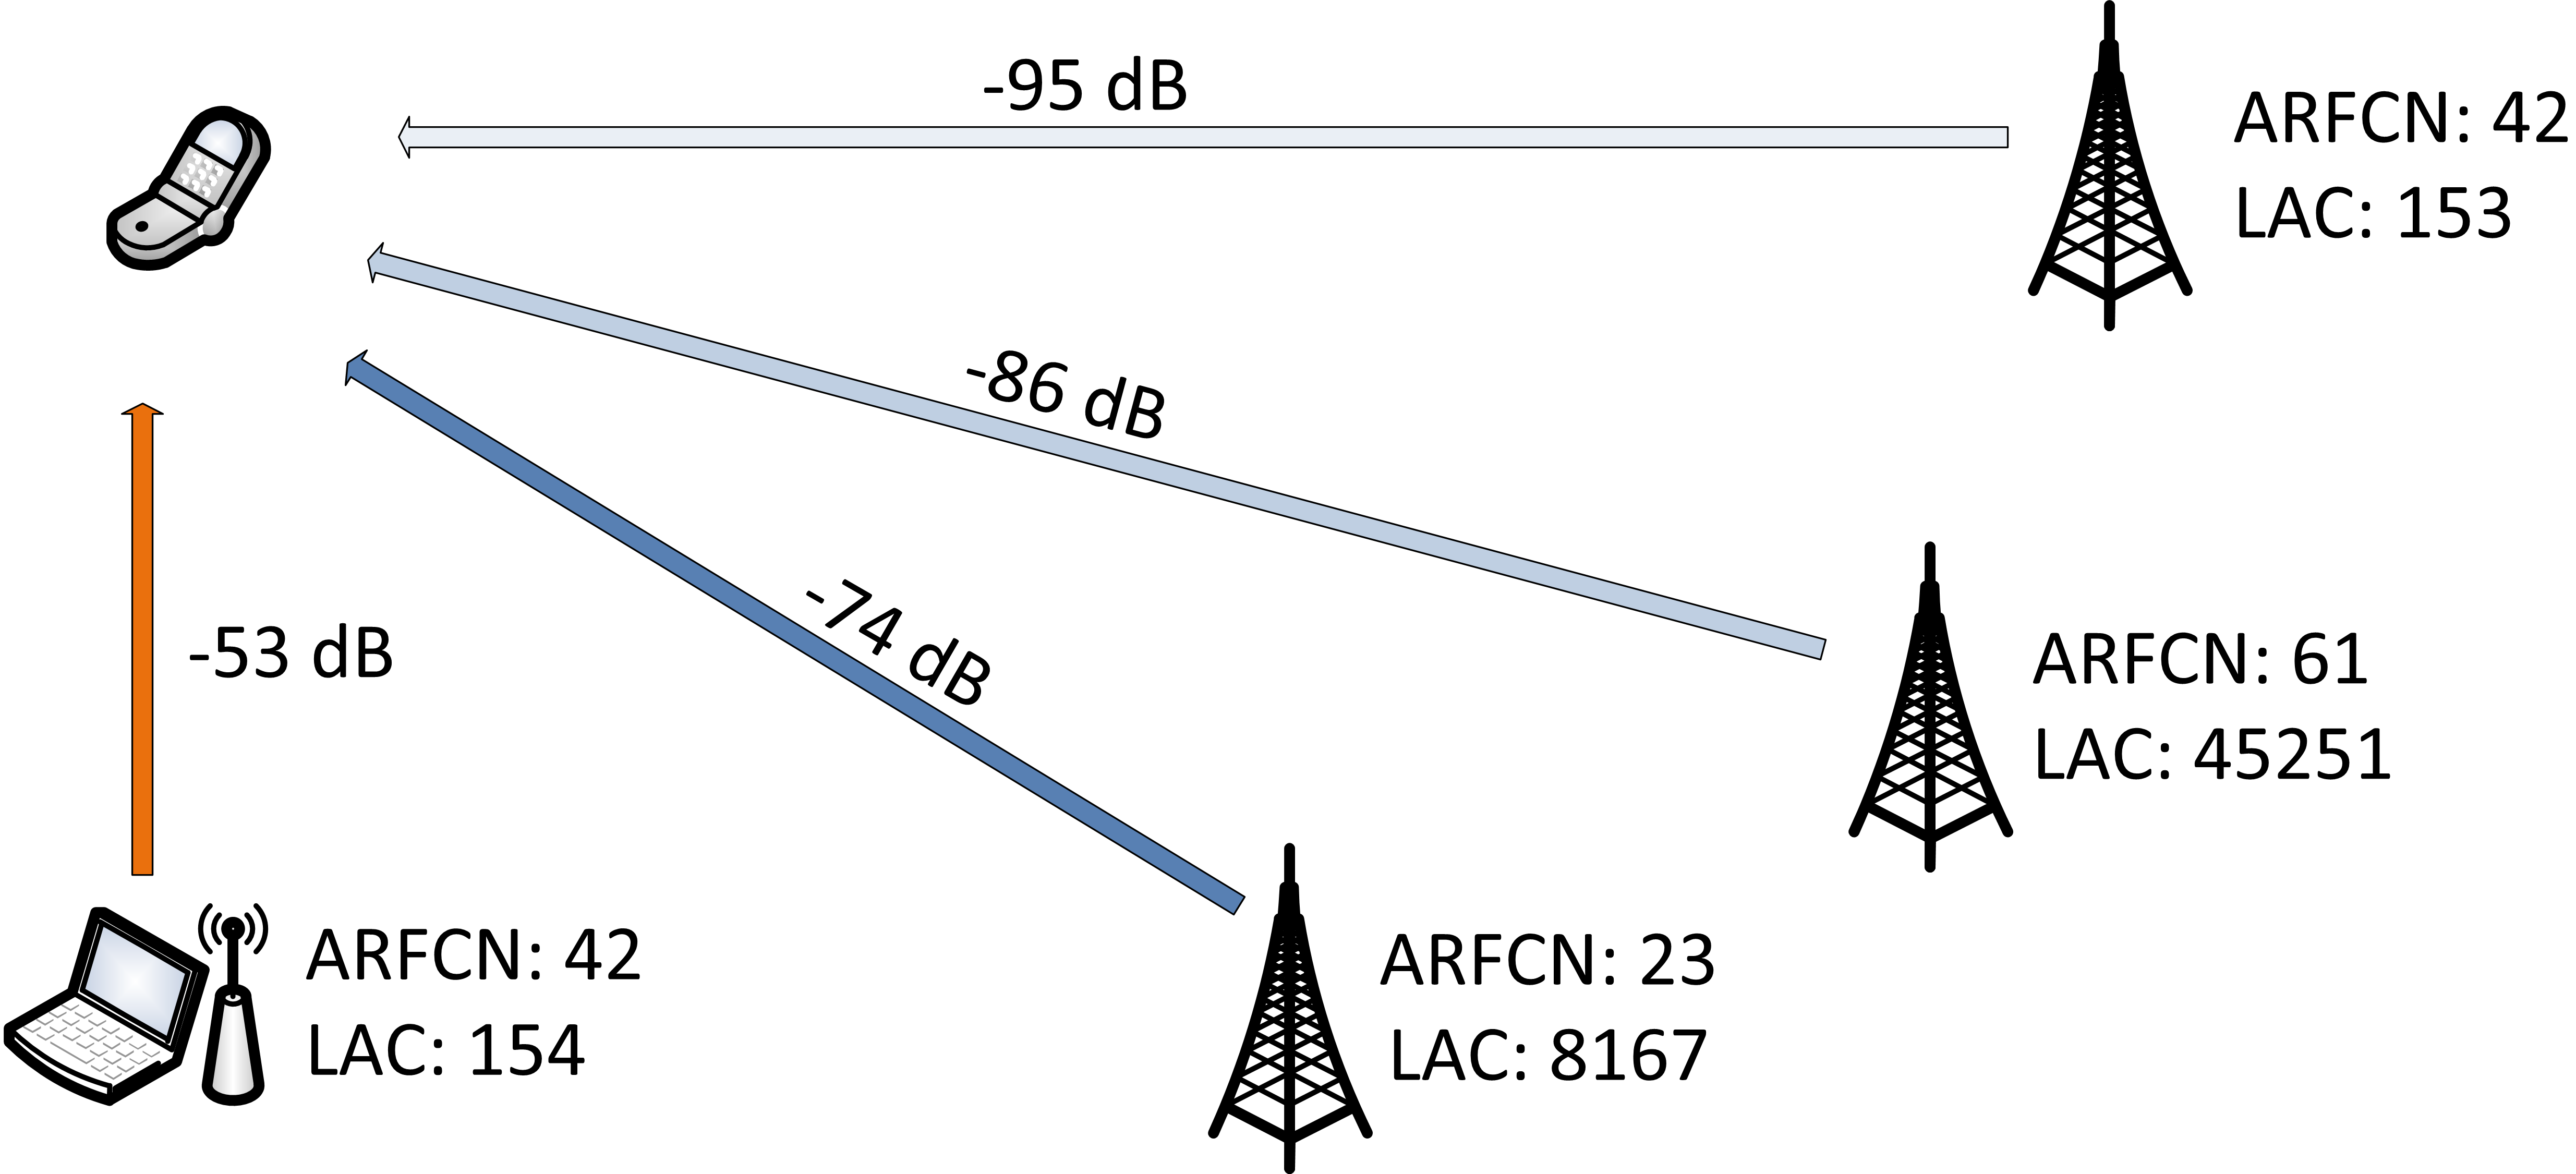
\includegraphics{../Images/replace_attack}
\caption{Takeover attack of an IMSI catcher on a base station.}
\label{fig:takeover_attack}
\end{figure}

Due to its strong increase in reception and the change in the \gls{lac} the IMSI catcher cell obtained a 'Critical' status immediately after it had been scanned a second time.
Also due to this fact the reception level differed too much from the interval that had been measured for this Cell ID  in the Local Area Database and received as a result also a 'Critical' rating from the respective rule.
User Mode did not start a PCH scan since the evaluation had already been 'Critical'.